\section{شبکه‌ی نورون‌های چرخنده}
در این مدل به جای آن که برای شبکه خود از مدل انباشت-شلیک استفاده کنیم از مدل چرخنده استفاده می‌کنیم. در این مدل نورون‌های ما مانند دونده‌هایی به دور میدان مثلثاتی می‌دوند. ما نقطه‌ی فاز $\pi$ را به عنوان علامت برای این دونده‌ها قرار دادیم. هر زمان که دونده‌ای از علامت خود گذشت یک تیزه برای او درنظرمی‌گیریم و بلافاصله او را به فاز $-\pi$ باز می‌گردانیم.\\

برای توصیف فاز هر نورون از معادلات زیر استفاده می‌کنیم:
\begin{tcolorbox}
	\begin{equation}
		\begin{cases}
			\dot{\theta_i}=I_i - cos(\theta_i) - g E, \hspace{2ex} - 5\pi/2 \leq \theta_i \leq \pi \\
			\dot{E} = M - \alpha E\\
			\dot{M} = -  \alpha M + \frac{ \alpha^{2} }{N} \sum_{n|tـn<t} \delta(t - t_n - t_d)
		\end{cases}
	\end{equation}
	\begin{enumerate}[-]
		\item $\theta_i$:
		مشخص کننده‌ی فاز هر نورون. این فاز میان دو لبه در حال حیات است. کوچکترین کران بالای آن همان حالت آستانه در $\pi$ است و بزرگترین کران پایین آن نگه‌دارنده‌ای است که از ریزش نورون‌ها جلوگیری می‌کند.
		\item $E$:
		میدانی است که شدت فعالیت شبکه را نشان می‌دهد.
		\item $M$:
		یک پارامتر فرعی که در حل معادله دیفرانسیل مرتبه دوم به دو معادله‌ی تحول مرتبه اول ما را یاری کرده است.
	\end{enumerate}
\end{tcolorbox}

\زیرقسمت{آهنگ تیزه زدن}
برای نورونی تنها که پویایی از جنس چرخنده دارد؛ دوره‌ی تناوب تیزه زدن آن بر حسب مجموع جریان ورودی‌ رفتاری مطابق زیر دارد \cite{safaeesirat2020critical}:

\begin{align}
	T = \frac{2\pi}{\sqrt{I^2 - 1}}
\end{align}
این به این معناست که مدل چرخنده و انباشت‌وشلیک اگر چه هر دو با افزایش جریان، بسامد تیزه زدنشان افزایش می‌یابد اما رفتار تغییر آن به دو گونه‌ی متفاوت صورت می‌پذیرد. این نکته‌ی مهمی است که در هنگام مقایسه‌ی دو مدل باید به خاطر داشته باشیم.

\زیرقسمت{نشانگر توسعه یافته‌ی تشخیص همگامی}
برای تشخیص هم‌گامی از یک پارامتر دیگری که در این مقاله \cite{safaeesirat2020critical}  توسط نویسندگان ابداع شده‌است؛ بهره می‌بریم.

\begin{equation}
	s =  \braket{ \big[ \frac{1}{N_a}\sum_{i_a} sin(\theta_{i_a}) \big]^{2}}_t
	\label{eq:saman_amin_param}
\end{equation}
میانگین‌گیری بالا روی ۱۰۰۰ گام آخر زمانی انجام می‌شود. این فاصله زمانی باید حتما بزرگ‌تر از گام‌های زمانی تحول ریزمقیاس آن باشد. همچنین برای این متوسط‌گیری نورون‌هایی را مدنظر می‌گیریم که در منطقه ی فعال قرار گرفته‌اند. منطقه‌ی فعال، سمت چپ دایره مثلثاتی است.
\subsection{شبیه‌سازی}
ثوابت مسئله را به گونه‌ی زیر انتخاب می‌کنیم.
\begin{tcolorbox}[colback=green!5!white,colframe=green!75!black]
	\begin{enumerate}[*]
		\item
		$\alpha = 20\, s^{-1}$
		\item
		جریان‌های تصادفی خارجی نورون‌ها از اعضای بازه‌ی $(9.5,13.5)$ انتخاب می‌شوند. این بازه به گونه‌ای انتخاب شده است که نورون خاموشی در سامانه وجود نداشته باشد.
		\item
		$N = 10000$
		\item
		$t_d = 0.1\, s$ 
	\end{enumerate}
\end{tcolorbox}
حال شبکه‌ی خود را به ازای قدرت اتصال‌های مختلف اجرا می‌کنیم تا مجددا تحقیق کنیم که چگونه تغییر در قدرت اتصال $g$ می‌تواند باعث شود تا تغییر فاز از ناهم‌گامی به هم‌گامی رخ دهد. برای مشاهده‌ی دفترچه شبیه‌سازی به آدرس 
\href{run://..//scripts//rotational_model}{مسئله همگامی برای مدل چرخنده}
مراجعه کنید.

\subsection{نتایج }
مرتبه‌ی اجرای این الگورتیم خطی است و برای یک شبکه شامل ۱۰۰۰ نورون و برای ۱۰۰۰۰ گام شبیه‌سازی زمانی در حدود ۴ ثانیه به طول می‌انجامد. 


\subsubsection{در جستجوی تغییرفاز}
پس از رصد کردن تغییرات رفتار سیستم بر حسب قدرت مهار نورون‌ها، تغییر فاز مانند مدل قبلی مشاهده شد اما مکان تغییر فاز تغییر کرد و حول $g=30$ قرارگرفت. این تغییر فاز در دو شکل \ref{fig:sigma_rotational} و \ref{fig:amin_saman_rotational}  قابل مشاهده‌است.
\begin{figure}
	\centering
	\includegraphics[width = 10 cm]{../scripts/all_neurons_model_in_one_place/Rotational_ensembles/N10000_T100_I9.5_13.5_cluster_computed/sigma_g_0.1_65.png}
	\caption{پهنای جریان یک سامانه چرخنده با ده هزار نورون}
	\label{fig:sigma_rotational}
\end{figure}

\begin{figure}
	\centering
	\includegraphics[width = 10 cm]{../scripts/all_neurons_model_in_one_place/Rotational_ensembles/N10000_T100_I9.5_13.5_cluster_computed/amin_saman_param_g_0.1_65.png}
	\caption{پارامتر نظم تعریف شده در رابطه \ref{eq:saman_amin_param} برای مدل چرخنده }
	\label{fig:amin_saman_rotational}
\end{figure}


\subsubsection{فاصله زمانی بین تیزه‌ها}
حال که دیدیم برخی نورون‌ها همواره خاموش می‌مانند و یا به عبارتی دوره‌ی تیزه زدن آن‌ها بینهایت است؛ خوب است که دوره‌ی تیزه زدن‌های نورون‌های دیگر را نیز بررسی کنیم. شکل \ref{fig:interspikes_rotational} این شکل نمایان‌گر آن است که توزیع دوره‌ها به توزیع بی‌توانی و رفتار بی‌مقیاس نزدیک است.\\
همچنین توجه کنیم که با افزایش ضریب تاثیر رفتار توانی آن‌ها تغییر نمی‌کند. تنها تفاوت در چگونگی انتخاب جایگاه‌های روی خط است. هر چه ضریب تاثیر بزرگتر می‌شود نورون‌ها فاصله‌ی زمانی تیزه‌های بزرگتری را اتخاذ می‌کنند.
\\
با این مشاهده، کنجکاو می‌شویم تا نمای بحرانی را برای آن حساب کنیم. در شکل \ref{fig:interspikes_rotational_trending_line} با گذراندن یک خط بر داده‌های بدست آمده از شبکه‌ای با قدرت مهار ۲۰ را می‌بینیم.

\begin{figure}[h]
	\centering
	\includegraphics[width = 10 cm]{../scripts/all_neurons_model_in_one_place/Rotational_ensembles/N10000_T100_I9.5_13.5_cluster_computed/mean_spiking_persiods_g_0.1_65.png}
	\caption{فاصله‌ی زمانی بین تیزه زدن‌ها}
	\label{fig:interspikes_rotational}
\end{figure}

\begin{figure}[h]
	\centering
	\includegraphics[width = 10 cm]{../scripts/all_neurons_model_in_one_place/Rotational_ensembles/N10000_T100_I9.5_13.5_cluster_computed/mean_spiking_persiods_with_trending_line_g_0.1_65.png}
	\caption{محاسبه‌ی نمای بحرانی}
	\label{fig:interspikes_rotational_trending_line}
\end{figure}


\subsubsection{فعالیت شبکه}
همان طور که دیدیم تعدادی از نورون‌ها در شبکه به حالت خاموش درمی‌آیند. قابل حدس است که اگر جمعیتی خاموش در شبکه داشته باشیم؛ احتمالا آنهایی هستند که جریان تصادفی اولیه آن‌ها از بقیه کمتر است. برای تحقیق این حدس لازم است تا تعداد تیزه‌های نورون‌های شبکه را بر حسب جریان تصادفی اولیه آنها مرتب کنیم. شکل \ref{fig:spikes_num_vs_background_current} نشانگر سامانه‌ای از ده هزار نورون است که با قدرت $g=50$ روی هم تاثیر می‌گذارند. لازم به ذکر است که این رفتار در فاز هم‌گام قابل مشاهده است. در فاز ناهم‌گام تمام نورون‌ها که از هم تاثیر کمتری می‌پذیرند؛ فعال هستند.


\begin{figure}[h]
	\centering
	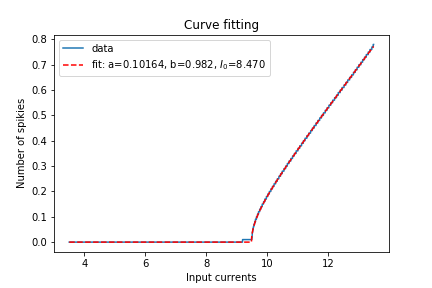
\includegraphics[width = 10 cm]{figs/Rotational/spikies_num_vs_input_fitted_curve_g50_input_3.5_13.5.png}
	\caption{تعداد تیزه بر حسب جریان تصادفی برای سامانه‌ای با ده هزار نورون و ضریب تاثیر $g=50$}
	\label{fig:spikes_num_vs_background_current}
\end{figure}

تعداد تیزه‌های کل شبکه رابطه‌ی مستقیمی با جریان خارجی جاری در شبکه دارد. می‌توانیم با محاسبات تحلیلی نیز به شکل بدست آمده از شبیه‌سازی عددی نزدیک شویم:

\begin{align}
	\begin{cases}
		I_{in} &= -g \int_{a_{min}}^{a_{max}} p(a) f(a + I_{in}) da \\
		f(a) &= \frac{\sqrt{a^2 - 1}}{2\pi}
	\end{cases}
	\label{eq:analytical_input_current}
\end{align}

در رابطه \ref{eq:analytical_input_current} ، $f(a)$ تابع فعالیت (تعداد تیزه بر ثانیه) تک نورون بر حسب جریان کل ورودی آن است. همچنین $I_{in}$ تمام جریان خارجی جاری در شبکه است.\\
حل این رابطه کمی دشوار است زیرا جریان کل را بر حسب خودش محاسبه کرده است. اما از آنجایی که در انتگرال‌ده تنها یک جابجایی ثابت رخداده است؛ صورت کلی پاسخ انتگرال تغییر نمی‌کند و به صورت زیر بدست خواهد آمد.
\begin{align}
	I_{in} = \frac{-g}{2} (-a \sqrt{-1 + a^2} + log(a + \sqrt{-1 + a^2})) \Big|_{a_{min} + I_{in}}^{a_{max} + I_{in}}
\end{align}
\زیرقسمت{پهن‌کردن قالی صفحه‌ی فاز}
در قسمت‌های پیشین تنها به مطالعه‌ی تاثیر ضریب اتصال در تغییرفاز پرداختیم و زمان تاخیر را تنها در $t_d = 0.1 s$ خلاصه کردیم. حال اجازه دهید تا به تاخیر نیز اجازه‌ی تغییر دهیم. در ادامه‌ی این قسمت از نوشتارمان، به فرش‌کردن صفحه‌ی فاز خود خواهیم پرداخت. امید است که چهره‌ی تمام نمای سامانه‌ بر صورت این قالی نقش بندد.\\


\زیرزیرقسمت{قالی انحراف از معیار میدان}
در شکل \ref{fig:rot_g_d_phase_space} مشاهده می‌کنیم که شدت هم‌گامی در هر کدام از هنگردهای سامانه چقدر است. بنظر می‌رسد که با افزایش زمان تاخیر و ضریب تاثیر همگامی قدرت پیدا می‌کند و هر دو در ظهور این رفتار شریک هستند.
\begin{figure}[h]
	\centering
	\includegraphics[width = 15 cm]{../scripts/all_neurons_model_in_one_place/Rotational_ensembles/N10000_T100_I9.5_13.5_cluster_computed/sigma_phase_space.png}
	\caption{صفحه‌ی فاز مربوط به سامانه‌ی نورون‌های چرخنده}
	\label{fig:rot_g_d_phase_space}
\end{figure}
